\documentclass[11pt]{article} % use larger type; default would be 10pt

\usepackage[utf8]{inputenc} % set input encoding (not needed with XeLaTeX)


\usepackage{geometry} % to change the page dimensions
\geometry{a4paper} % or letterpaper (US) or a5paper or....

\usepackage{graphicx} % support the \includegraphics command and options
\usepackage{amsmath}


\usepackage{booktabs} % for much better looking tables
\usepackage{array} % for better arrays (eg matrices) in maths
\usepackage{paralist} % very flexible & customisable lists (eg. enumerate/itemize, etc.)
\usepackage{verbatim} % adds environment for commenting out blocks of text & for better verbatim
\usepackage{subfig} % make it possible to include more than one captioned figure/table in a single float

\usepackage{fancyhdr} % This should be set AFTER setting up the page geometry
\pagestyle{fancy} % options: empty , plain , fancy
\renewcommand{\headrulewidth}{0pt} % customise the layout...
\lhead{}\chead{}\rhead{}
\lfoot{}\cfoot{\thepage}\rfoot{}

\usepackage{sectsty}
\allsectionsfont{\sffamily\mdseries\upshape} % (See the fntguide.pdf for font help)

\usepackage[nottoc,notlof,notlot]{tocbibind} % Put the bibliography in the ToC
\usepackage[titles,subfigure]{tocloft} % Alter the style of the Table of Contents
\renewcommand{\cftsecfont}{\rmfamily\mdseries\upshape}
\renewcommand{\cftsecpagefont}{\rmfamily\mdseries\upshape} % No bold!
\newcommand{\strong}[1]{\textbf{#1}}
\newcommand{\code}[1]{\texttt{#1}}
\newcommand{\st}{$^{\text{st}\ }$}
\newcommand{\nd}{$^{\text{nd}\ }$}
\newcommand{\rd}{$^{\text{rd}\ }$}
\newcommand{\nth}{$^{\text{th}\ }$}

\title{Assignment 4}
\author{Nathan Jervis}

\begin{document}
\maketitle

\section{Question 4.4}

\subsection{Part A}

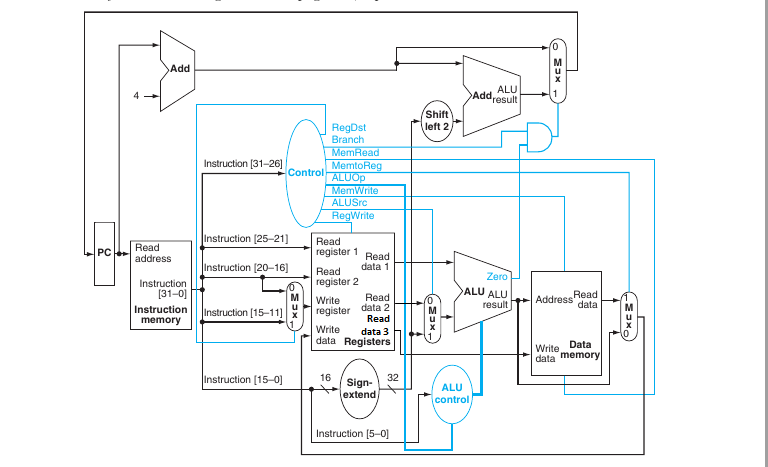
\includegraphics[width=\textwidth]{CPU3.png}

We can re-use the write register selection as the selection for a 3\rd read register. This read register is used as the write data now, instead of the 2\nd one like the previous diagram. We can make this transistion since the only opcode which currently uses that data line is \code{sw}. All we need to do is ensure that for \code{sw} the \strong{RegDst} control pin is set to 0, so the [20-16] part of the opcode is used as the write register selection. Since we've already repurposed this to read into the new 3\rd register line, it will still output the same information to the \emph{write data} section of the memory unit. \code{swr} will have \strong{RegDst} set to 1, and will therefore use the [15-11] part of the opcode to select which register to write.

Adding this new command \code{swr} requires reading from a 3\rd register, but it does not need any additional control lines, and doesn't even add new wiring to the circuit (besides what's required inside the register file to read from a 3\rd register that is). 

\subsection{Part B}

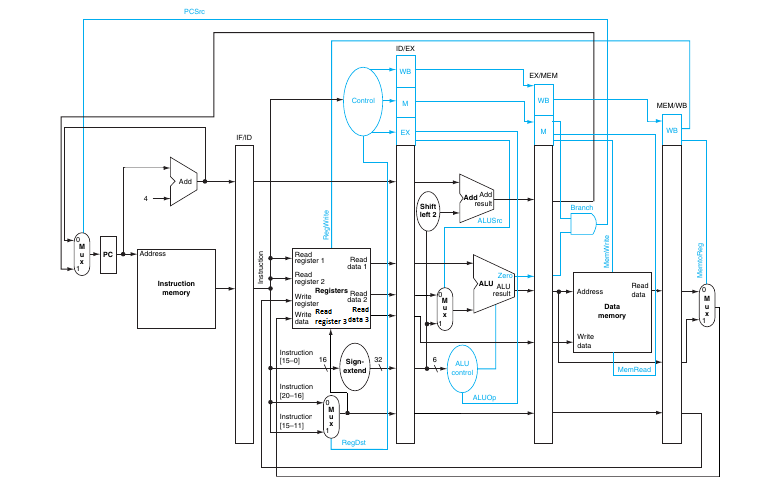
\includegraphics[width=\textwidth]{pipelineCPU4.png}

The pipelined version requires a few more changes. We can't simply re-use the write register selector, since in the original diagram it's not known until the \emph{Execute} stage. We alter it to move the calculation of which register to use to the \emph{Instruction Decode} stage, so we can select the read register. This actually saves us a pipeline register which we can use to store the result of the 3\rd read register.

In this version we do change the circuit in a more major way, however all of the additional logic is in the \emph{Instruction Decode} stage, which is usually seen as one of the shorter stages, so making it take longer might not even increase the time for each pipeline stage, since it's normally waiting for \emph{Execute} to complete.

Whether \code{swr} is worth implementing or not really would come down to seeing if it extends the time of \emph{Instruction Decode} past the time it's waiting, and if it does, if saving the instruction calls offsets the additional time added. However \code{lwr} can be implemented without any significant changes to the CPU (simply adding a new entry to the \strong{Control} table logic), and so can be easily implemented. If \code{swr} is deemed to be too expensive it can be implemented as a pseudo-instruction such that \code{swr \$t0, \$t1, \$t2} compiles to:

\begin{verbatim}
    add $at, $t1, $t2
    sw $$t0 0($at)
\end{verbatim}

In this way you'd be able to have the benefit of \code{lwr} without any of the complexity introduced by \code{swr}.

\subsection{Part C}

There are no new hazards introduced, just slightly different things to look out for. \code{lwr} has basically the same hazards as any arithmetic operation such as \code{add} (it may make a difference for optimization sake that \code{lwr} loads from memory, ie to prefetch it, but it doesn't introduce new hazards). \code{swr} is a little bit of an oddball since it now reads from a 3\rd register, and this will have to be kept in mind, but it doesn't introduce any new types of hazards, just a 3\rd spot to check for read hazards in this instruction (whereas normally it'd only check the 3\rd register for write hazards).


\section{Question 4.5}

\emph{Note: I'm assuming for these questions we're using the original CPU as in the textbook, and not the new one with \code{swr} and \code{lwr}}

\subsection{Part A}

Cross talk between \emph{RegDst} and \emph{MemWrite}, causing them to be the logical \strong{AND} of the 2 inputs. The only case when \emph{MemWrite} is 1 is when the \code{sw} opcode is used. In this case \emph{RegDst} is 0, which means with this cross-talk both \emph{RegDst} and \emph{MemWrite} will always be \code{0/false} which will cause disastrous consequences for code (as \code{sw} will never actually write it's data, and all registers which are supposed to use the 3\rd register to write to end up using the 2\nd instead, which is all \emph{r-format} instructions. In order to detect this problem the following code can be used:

\begin{verbatim}
    #load in 1 to $t0
    #immediate value functions expect RegDst to be 0, so they still work
    ori $t0, $zero, 1
    ori $t1, $zero, 2 #load in 2 to $t1
    ori $t2, $zero, 3 #load in 3 to $t2
    #add $t0 and $t1 and store in $t0
    #on an affected system, the CPU will store the result in $t1 instead
    add $t0, $t0, $t1 
    #the only possible way 2 could equal 3 would be on the broken system
    beq $t1, $t2, Fault 
\end{verbatim}

\subsection{Part B}

Cross talk between \emph{RegDst} and \emph{MemWrite}, causing them to be the logical \strong{OR} of the 2 inputs. This means that \code{sw} will now work correctly, but every instruction that sets \emph{RegDst} to 1 will also write to memory. In particular the \emph{r-format} instructions all set \emph{RegDst} to 1, so they will also write the 2\nd read register to memory (the memory location determined by the result of the operation). In order to detect this problem the following code can be used:

\begin{verbatim}
    #translated to lui and ori, both of which are I-format 
    #and not affected by this bug
    #temp is any temporary memory location that is non-zero
    li $t0, temp 
    ori $t1, $zero, 0#load 0 into t1
    sw $t1, 0($t0) #store 0 into the temp memory location
    #if the machine has this bug then it'll store 2\nd read register 
    #(which is the address of temp) into the location determined by the result 
    #(which is also the address of temp)
    #this basically means that the temp memory location now contains it's own 
    #address (which is why it must be non-zero)
    add $t2, $t1, $t0 
    lw $t2, 0($t0) #load temp back in
    beq $t2, $t1, end #check if temp is still 0
    j fault #the only way we're here is if temp was altered between sw and lw
end:   #if we reach this point we're successful, so the rest of the code can go here
\end{verbatim}

\subsection{Part C}

Cross talk between the last segment and the \emph{EX} segment of the \emph{RegWrite} causing them to be the logical \strong{AND} of the 2 inputs. This means that an instruction will only write back into the register if the instruction 2 cycles behind it is also writing back into a register (ie both are \emph{r-format} or \code{lw} instructions). Depending on the cross-talk it could also mean that the \emph{RegWrite} control bit could be affect by the instruction 2 cycles earlier. (For simplicity sake, I'm going to assume that the first 2 instructions don't get affected by the state of the \emph{RegWrite} line 2 cycles before them (which would make it completely undefined)). The following code might detect the problem:

\begin{verbatim}
    #this instruction write backs succesfully
    ori $t0, $zero, 2 #load 2 into t0
    #this instruction writes back succesfully
    ori $t1, $zero, 2 $load 2 into t1
    #this instruction fails on a problematic machine
    ori $t0, $zero, 3 #load 3 into t0
    #this is basically a nop to ensure instruction 2 works
    ori $t0, $t0, 0
    #this serves a dual purpose, it compares t0 and t1
    #and it also screws up isntruction 3 on a problem machine
    beq $t0, $t1, fault # go to fault if instruction 3 didn't work
\end{verbatim}

This code may not always work however, because depending on the implementation, it could have pipeline stalls. Simple stalls based on register usage could be avoided by adding the \code{ori $t0, $t0, 0} nop intermixed with regular \code{nop} depending on whether the instruction 2 prior should succeed or fail, but there will always be a chance that loading the instruction itself causes a cache miss, and stalls the pipeline. Also since the CPU can feel free to re-order instructions without dependencies, there is no saying that it won't re-order the program to make it execute completely differently.

\subsection{Part D}

Cross talk between the last segment and the \emph{EX} segment of the \emph{RegWrite} causing them to be the logical \strong{OR} of the 2 inputs. This means that the instruction will write back into the regiser if either it should write back, or the instruction 2 later should write back (again, depending on the nature of the cross talk, it could also be affected by instructions 2 prior, and again for simplicity I'm assuming the first 2 instructions aren't affected by the state of \emph{RegWrite} before the program starts). There is no code to detect it, since this cross-talk will only make things that aren't supposed to set RegWrite to have RegWrite set. This means \code{sw} and \code{beq}. However what gets written and where is undefined since \emph{MemToReg} and \emph{RegDst} are both undefined for those opcodes. So this means that either the result of the ALU, or the memory at the location of the result of the ALU could be written. This could be gotten around by making both of those the same (for the simple case, make them both zero), but which register they write to is undefined, and worse they could potentially write to a register that's part of the immediate value in the opcode. It would be very difficult to get around both of these problems, and considering how much any pipeline stalls would screw up the code (and since both \code{beq} and \code{sw} are very prone to causing stalls in unpredictable ways), it would be irresponsible to believe the effort would be worth it.

In short, if you believe your processor could have cross-talk here, it's not worth you time to diagnose it, go out and buy a new processor, they are super cheap.


\section{Question 4.6}

\begin{verbatim}
I1:      lw $t0, 4($s3)
I2:      addi $t0, $t0, 4
I3:      sw $t1, 0($t0)
I4:     add $t1, $t0, $t1
I5:     lw $t2, 12($s3)
I6:     addi $t2, $t2, -4
I7:     lw $t3, 8($t2)
I8:     sw $s3, 0($t1)
I9:     sw $t1, 0($t3)
\end{verbatim}

\subsection{Part A}

\begin{tabular}{c|c|c|c}
	Type & Register & Instruction 1 & Instruction 2\\\hline
	RAW & \$t0 & I1 & I2 \\
	WAW & \$t0 & I1 & I2 \\
	RAW & \$t0 & I2 & I3 \\
	WAR & \$s3 & I5 & I8 \\
	RAW & \$t1 & I3 & I4 \\
	WAW & \$t1 & I3 & I4 \\
	RAW & \$t1 & I4 & I8 \\
	WAR & \$t1 & I8 & I9 \\
	RAW & \$t2 & I6 & I7 \\
	RAW & \$t3 & I7 & I9 
\end{tabular}

\subsection{Part B}

\begin{verbatim}
    lw $t0, 4($s3)
    NOP #stall from RAW
    NOP
    addi $t0, $t0, 4
    NOP #stall from RAW
    NOP
    sw $t1, 0($t0)
    add $t1, $t0, $t1
    lw $t2, 12($s3)
    NOP #stall from RAW
    NOP
    addi $t2, $t2, -4
    NOP #stall from RAW
    NOP
    lw $t3, 8($t2)
    sw $s3, 0($t1)
    NOP #stall from RAW of $t3
    sw $t1, 0($t3)
\end{verbatim}

\subsection{Part C}

\begin{verbatim}
    lw $t0, 4($s3)
    NOP #stall from RAW
    NOP
    addi $t0, $t0, 4 #normally RAW, but can forward ALU-ALU
    sw $t1, 0($t0)
    add $t1, $t0, $t1
    lw $t2, 12($s3)
    NOP #stall from RAW
    NOP
    addi $t2, $t2, -4 #normally RAW, but can forward ALU-ALU
    lw $t3, 8($t2)
    sw $s3, 0($t1)
    NOP #stall from RAW of $t3
    sw $t1, 0($t3)
\end{verbatim}

\subsection{Part D}

\begin{verbatim}
    lw $t0, 4($s3) 
    NOP #stall from RAW, forward MEM-ALU (but still stalls once)
    addi $t0, $t0, 4 #normally RAW, but can forward ALU-ALU
    sw $t1, 0($t0)
    add $t1, $t0, $t1
    lw $t2, 12($s3)
    NOP #stall from RAW, forward MEM-ALU (but still stalls once)
    addi $t2, $t2, -4 #normally RAW, but can forward ALU-ALU
    lw $t3, 8($t2)
    sw $s3, 0($t1) #normally RAWs stall, but MEM-ALU avoids 2nd stall
    sw $t1, 0($t3)
\end{verbatim}

\subsection{Part E}

\begin{tabular}{c|c|c|c}
Forwarding type & Cycle time & \# number of cycles & Total time\\\hline
No forwarding & 250ps & 18 & 4500ps \\
ALU-ALU forwarding & 280ps & 14 & 3920ps \\
Full forwarding & 300ps & 11 & 3300ps
\end{tabular}

\vspace{5mm}
Speedup by adding full forwarding to a pipeline with no forwarding:
\[
	1 - \frac{\text{Old Time}}{\text{New Time}} = 1 - \frac{4500}{3300} = 1 - 1.3636 = 0.3636 = 36\%
\]

Speedup by adding full forwarding to a pipeline with ALU-ALU forwarding
\[
	1 - \frac{\text{Old Time}}{\text{New Time}} = 1 - \frac{3920}{3300} = 1 - 1.1879 = 0.1879 = 19\%
\]

\subsection{Part F}

\begin{verbatim}
    lw $t2, 12($s3)
    lw $t0, 4($s3)
    #RAW hazard with $t2
    addi $t2, $t2, -4
    addi $t0, $t0, 4
    #RAW hazard with $t2
    lw $t3, 8($t2)
    add $t1, $t0, $t1
    sw $t1, 0($t0) #this must read from $t1 before the previous writes to it
    #RAW haazard with $t1
    sw $s3, 0($t1)
    sw $t1, 0($t3)
\end{verbatim}

\subsection{Part G}

\begin{verbatim}
    lw $t2, 12($s3)
    lw $t0, 4($s3)
    NOP
    addi $t2, $t2, -4
    addi $t0, $t0, 4
    NOP
    lw $t3, 8($t2)
    add $t1, $t0, $t1
    sw $t1, 0($t0) #this must read from $t1 before the previous writes to it
    NOP
    sw $s3, 0($t1)
    sw $t1, 0($t3)
\end{verbatim}

subsection{Part H}

\begin{tabular}{c|c|c|c}
Forwarding type & Cycle time & \# number of cycles & Total time\\\hline
No forwarding & 250ps & 12 & 3000ps
\end{tabular}

Re-ordering it can save a significant amount of time without even having to implement forwarding. If forwarding was implemented here, then all the remaining NOPs could be removed, and it'd be down to 9 instructions (and take a total of 2700ps)

\section{Bonus Part}

\emph{No this bonus question wasn't ever given. I just decided to give it to myself because it intrigued me.}\\

\code{lwr} and \code{swr} can be extended to use the \strong{shamt} to shift one of the operands. In this way the following instruction sequence:

\begin{verbatim}
    #s0 contains the base array address
    #s1 contains the index, needs to be multipled by 4
    #s2 contains the information to write
    sll $t0, $s1, 2
    add $t0, $s0, $t0
    sw $s2, 0($t0)
\end{verbatim}

Can be transformed into just \code{swr \$s2, \$s1, \$s0, 2} which adds the array base to the index shifted by 2. This not only saves 2 instructions, it also saves 1 temporary register. In order to do this we need to modify the pipelined CPU in the following way:

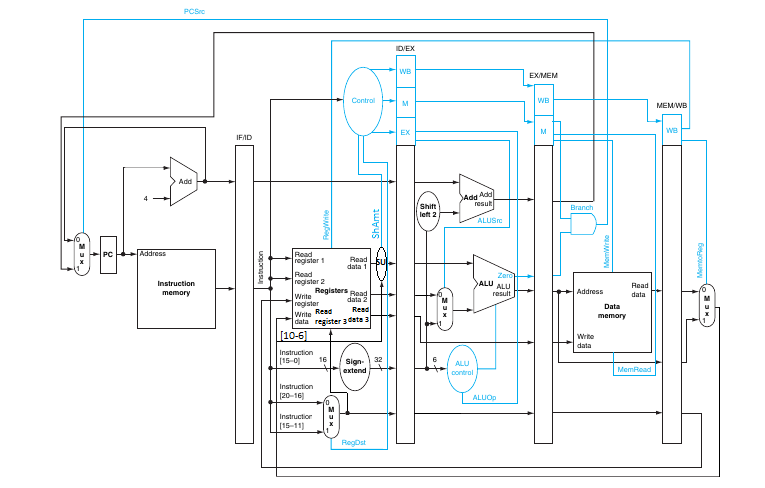
\includegraphics[width=\textwidth]{pipelineCPU5.png}

This adds to the existing modified CPU a new component which shifts the first read register by the amount given by \strong{shamt} ([10-6]) if the \emph{ShAmt} control pin is set (which is set to true for all \emph{r-format} instructions, it could probably be replaced by \emph{RegDst} if a new control pin is not wanted). This enables us to shift the one register, add it to the 2nd and then use that as the address to use.

By adding this to all \emph{r-format} instructions, other instructions can use it as well, enabling quite a few other optimizations, including the following:

\subsection{Index Offsets}

This is the one given above, basically can reduce a 3 instruction, with one temprorary register sequence to 1 instruction with no temporary registers. In addition to this it can also be used to calculate addresses for use by pointers. In this way it's essentially the \code{LEA} instrution in X86, except it can't add a constant, so many of the same tricks can be used.

\subsection{Multiply by 2n+1}

In order to multiply a number by a constant, MIPs requires 3 instructions:

\begin{verbatim}
    #s0 contains the number to be multipled, and stored in s1
    ori $t0, $zero, 3
    mult $t0, $s0
    mflo $s1
\end{verbatim}

Worse is that the multiply instruction is quite expensive and may require several cycles. In our CPU here, it probably isn't even implemented. Luckily it can be hardcoded. For powers of 2 it's quite easy, just do something like this (for $\times 4$) \code{sll \$s1, \$s0, 2}. However for something like $\times 5$ something like the following has to be used:

\begin{verbatim}
    #again s0 contains the number to be multipled and stored in s1
    sll $s1, $s0, 2
    add $s1, $s1, $s0
\end{verbatim}

Which is a 2-instruction sequence that we can now optimize to a single instruction with \code{add \$s1, \$s0, \$s0, 2} (which adds it to itself shifted by 2), so now we can multiply by $2n+1$ in a single instruction as well.\\

Similarily we can use sub to multiply by $2n-1$ with \code{sub \$s1, \$s0, \$s0, 2} (which subtracts \$s0 from itself shifted by 2).

\subsection{Mask and Move bit operation}

Oftentimes people pack information into a single word in order to store it more compactly. Let's say we have a 32-bit word that contains 32 flags (bit values for \code{true}/\code{false}), the following operation is needed to get the 5\nth flag for instance (using a mask):

\begin{verbatim}
    #s0 contains the flag word
    #s1 contains the mask
    #s2 contains the result
    sll $s2, $s0, -5
    and $s2, $s2, $s1
\end{verbatim}

This means it requires 2 operations for a fairly trivial operation (bit masking is used for all sort of situations, for instance on the new iOS device, the upper 32 bits of the 64 bit pointer is used for refernce counting as well as other additional information. This means using this pointer requires bit masking). With the new modifications this can be done in a single operation (assuming the mask is already loaded).

\begin{verbatim}
    #s0 contains the flag word
    #s1 contains the mask
    #s2 contains the result
    and $s2, $s2, $s1, -5
\end{verbatim}

This saves a single operation for the 2-operation sequence, but the impact could be even greater, since it is now a single operation to get various sections out of a word, compressing several things into a single word is a much more plausible thing to do. If this optimization causes it to be plausible to store entire structures, the optimization could be even better. Let's say we have the following C struct:

\begin{verbatim}
    struct
    {
        c1: char;
        c2: char;
        c3: char;
        b1: bool;
        b2: bool;
        b3: bool;
        b4: bool;
        b5: bool;
        b6: bool;
        b7: bool;
        b8: bool;
    }
\end{verbatim}

That is a structure storing 3 chars, and 8 boolean values, without bit masking this would take a word for each field, which is 11 words. Using bit masking this would only take 1 word, at the expense of an additional operation to access each value. By enabling the \strong{shamt} and making it take just one instead of 2, that's a very real performance difference for accessing fields, and could make this possible to do. In return we now have only 1 word, and the cache only needs to be an 11\nth of the size in order to get the same performance (and for the same cache size, we'd get much better performance). Alternatively you could use \code{lb} and \code{sb} to grab individual bytes (and this would only take 11 bytes instead, or 3 words), but if mutliple fields are needed, this is wasteful (as to grab 4 fields, you'd need 4 loads instead of 1). 

If systems use space in the pointer to store a reference count, this optimization makes reference counting much faster, and since working with pointers is a very common operation, this would cause very real performance gains.

\subsection{Analysis of impact}

This adds additional work which must be done to the 1\st read register, but shifts are fast (each calculation for each bit is independent of the rest) and it's done in the \emph{Instruction Decode} stage. This work can also be done while determining the 3\rd read register is done, so it probably doesn't have any more of an impact than simply adding \code{swr} does. The extra control pin can probably be replaced by the existing \code{RegDst} control pin (as long as the undefined states for non-\emph{r-format} instructions is set to \code{false}). In return several very nice optimizations can be made, including ones that could speed up runtimes (reference counting ones in particular) by a very real amount.

\end{document}

